% !TEX TS-program = xelatex
% !TEX encoding = UTF-8 Unicode
% !Mode:: "TeX:UTF-8"

\documentclass{resume}
\usepackage{zh_CN-Adobefonts_external} % Simplified Chinese support using external fonts (./fonts/zh_CN-Adobe/)
%\usepackage{zh_CN-Adobefonts_internal} % Simplified Chinese support using system fonts
\usepackage{linespacing_fix} % Disable extra space before the next section
\usepackage{cite}
\usepackage{graphicx}
\usepackage{geometry}
\usepackage{multicol}
\usepackage{tabularray}
\usepackage{enumitem}
\usepackage{setspace}
\usepackage{hyperref}
\usepackage{xeCJK}
\usepackage{tabularx} % Automatically adjusted width tables
\usepackage{booktabs} % Nicer horizontal rules (top, mid, bottomrule)
\usepackage{array}    % For >{\raggedright\arraybackslash}
\usepackage{ifthen}
\usepackage{etoolbox} % Logical operators (OR/AND)
\usepackage{atveryend} % Run commands at the end of the document

\newwrite\namefile

%\setstretch{1.5}

% Development:5 ; Algorithm Engineer:0 ; Autonomous Driving Algorithms:10 ; Autonomous Driving Development:3 ; Gaming:1
\def\JobIndex{3}

%--------------
% Role configuration
%--------------

% Automatically compile the PDF according to \outputFileName
% 
% [Method 1: Python script (recommended)]
% 1. Run: python compile_resume.py
% 2. The script extracts the value of \outputFileName and compiles the document
% 
% [Method 2: Windows batch file]
% 1. Double-click: compile_resume.bat
% 
% [Method 3: TeXstudio user command]
% Option A (Python script):
% 1. Options -> Configure TeXstudio -> Build -> User Commands
% 2. Add a new command: C:\Users\chenguanbin\anaconda3\python.exe compile_resume.py
% python compile_resume.py does not work
% 3. Tools -> User -> Command X (or custom shortcut)
% 
% Option B (batch file, Windows only):
% 1. Options -> Configure TeXstudio -> Build -> User Commands
% 2. Add a new command: compile_resume.bat or cmd /c compile_resume.bat
% 3. Tools -> User -> Command X (or custom shortcut)
% 
% [Method 4: Manual compilation]
% xelatex -jobname=<value of \outputFileName> -synctex=1 -interaction=nonstopmode --shell-escape resume-zh_CN.tex
% Run twice to ensure references are correct

\def\outputFileName{GuangbinChen_Resume}

\ifcase\JobIndex
% x=0 (general/default)
\def\outputFileName{GuangbinChen_Resume_AlgorithmEngineer}
\or
% x=1 (miHoYo Development)
\def\outputFileName{GuangbinChen_Resume_Gaming}
\or
% x=2 (C++ Navigation Planning)
\def\outputFileName{GuangbinChen_C++Engineer_AutonomousDriving_Maps}
\or
% x=3 (XPENG)
\def\outputFileName{GuangbinChen_Resume_AutonomousDrivingDev}
\or
% x=4 (TikTok Client Android/iOS)
\def\outputFileName{GuangbinChen_TikTokClient(Android_iOS)}
\or
% x=5
\def\outputFileName{GuangbinChen_Resume_Development}
\or
% x=6
\def\outputFileName{GuangbinChen_Resume_AutonomousDrivingAlgorithms}
\or
% x=7
\def\outputFileName{GuangbinChen_Resume_TwoPages}
\or
% x=8
\def\outputFileName{GuangbinChen_Resume_LowLevel}
\or
% x=9
\def\outputFileName{GuangbinChen_Resume_Yajiang}
\or
% x=10
\def\outputFileName{GuangbinChen_Resume_AutonomousDrivingAlgorithms}
\else
% Default/error
\def\outputFileName{GuangbinChen_Resume_Error}
\fi

% Automatically rename the PDF after compilation
% Note: shell-escape must be enabled in TeXstudio
% 
% [Steps]
% 1. Open TeXstudio
% 2. Options -> Configure TeXstudio (Alt+O)
% 3. Select "Build" on the left
% 4. In the "Build Command" area, find the "XeLaTeX" command box
% 5. Append --shell-escape to the original command:
%    xelatex -synctex=1 -interaction=nonstopmode --shell-escape %.tex
% 6. Click OK to save
% 
% [Default command format]
% Original: xelatex -synctex=1 -interaction=nonstopmode %.tex
% New:      xelatex -synctex=1 -interaction=nonstopmode --shell-escape %.tex
% 
% Note: --shell-escape must be near the end of the command (before %.tex)
\AtEndDocument{%
  \IfFileExists{\jobname.pdf}{%
    \edef\tempjobname{\jobname}%
    \edef\tempoutputname{\outputFileName}%
    \edef\tempcmd{cp "\tempjobname.pdf" "\tempoutputname.pdf" 2>/dev/null || copy "\tempjobname.pdf" "\tempoutputname.pdf" 2>nul}%
    \immediate\write18{\tempcmd}%
  }{}%
}

%--------------
% Margin configuration
%--------------

% Adjust by 0.05 each time to fill exactly one page

\ifcase\JobIndex
% Case 0: default margins
\def\myMargin_0{1.5cm}
\geometry{a4paper,left=\myMargin_0,right=\myMargin_0,top=\myMargin_0,bottom=\myMargin_0}
\or
% Case 1: miHoYo
\def\myMargin_1{1.1cm}
\geometry{a4paper,left=\myMargin_1,right=\myMargin_1,top=\myMargin_1,bottom=\myMargin_1}
\or
% Case 2: Gaode C++ Navigation Engineer
\geometry{a4paper,hmargin=2.7cm,vmargin=2cm}
\or
% Case 3: XPENG
\geometry{a4paper,hmargin=2cm,vmargin=2.7cm}
\or
% Case 4: TikTok
\geometry{a4paper,hmargin=2.1cm,vmargin=3cm}
\or
% Case 5: Reserved
\geometry{a4paper,hmargin=2.1cm,vmargin=3cm}
\or
% Case 6: Reserved
\geometry{a4paper,hmargin=2.0cm,vmargin=4cm}
\or
% Case 7: Custom margins
\geometry{a4paper,hmargin=2.0cm,vmargin=4cm}
\or  % *** Fixed: \or between Case 7 and Case 8 ***
% Case 8: Reserved
\relax
\or
% Case 9: Reserved
\relax
\or
% Case 10: Custom margins
\def\myMargin_10{1.05cm}
\geometry{a4paper,left=\myMargin_10,right=\myMargin_10,top=\myMargin_10,bottom=\myMargin_10}
\or
% Case 11: Custom margins
\def\myMargin_11{0.95cm}
\geometry{a4paper,left=\myMargin_11,right=\myMargin_11,top=\myMargin_11,bottom=\myMargin_11}
\else
% Default/error: JobIndex > 11 or negative
\geometry{a4paper,margin=2.5cm}
\fi

\begin{document}
\ifthenelse{\equal{\JobIndex}{3}}{
	% XPENG: increase font size by 1pt
	\fontsize{11pt}{13.2pt}\selectfont
}{}
\pagenumbering{gobble} % suppress page numbers

%--------------
% Personal Information
%--------------

\begin{minipage}[t]{0.78\textwidth}
	\centering
	\name{\Huge Guangbin Chen}
	\vspace{0.5em}
	\contactInfo{(+86)15308638672}{congmingyige97@gmail.com}{Guangzhou, Guangdong}{}
	GitHub: \href{https://github.com/congmingyige?tab=repositories}{github.com/congmingyige} \quad|\quad 
	Blog: \href{https://www.cnblogs.com/cmyg}{cnblogs.com/cmyg}
	
	\ifcase\JobIndex
	\relax
	\or
	% Case 1: miHoYo
	%Position Applied: Game Client Tool Development
	\relax
	\or
	\relax
	\or
	%Position Applied: Autonomous Driving Software Development (Guangzhou)
	\relax
	\fi
	
	%\ifthenelse{\equal{\JobIndex}{3}}{
	%Position Applied: Autonomous Driving Software Development (Guangzhou)
	%}
\end{minipage}%
\begin{minipage}[t]{0.15\textwidth}
	\vspace{-2.4em}
	\begin{flushright}
		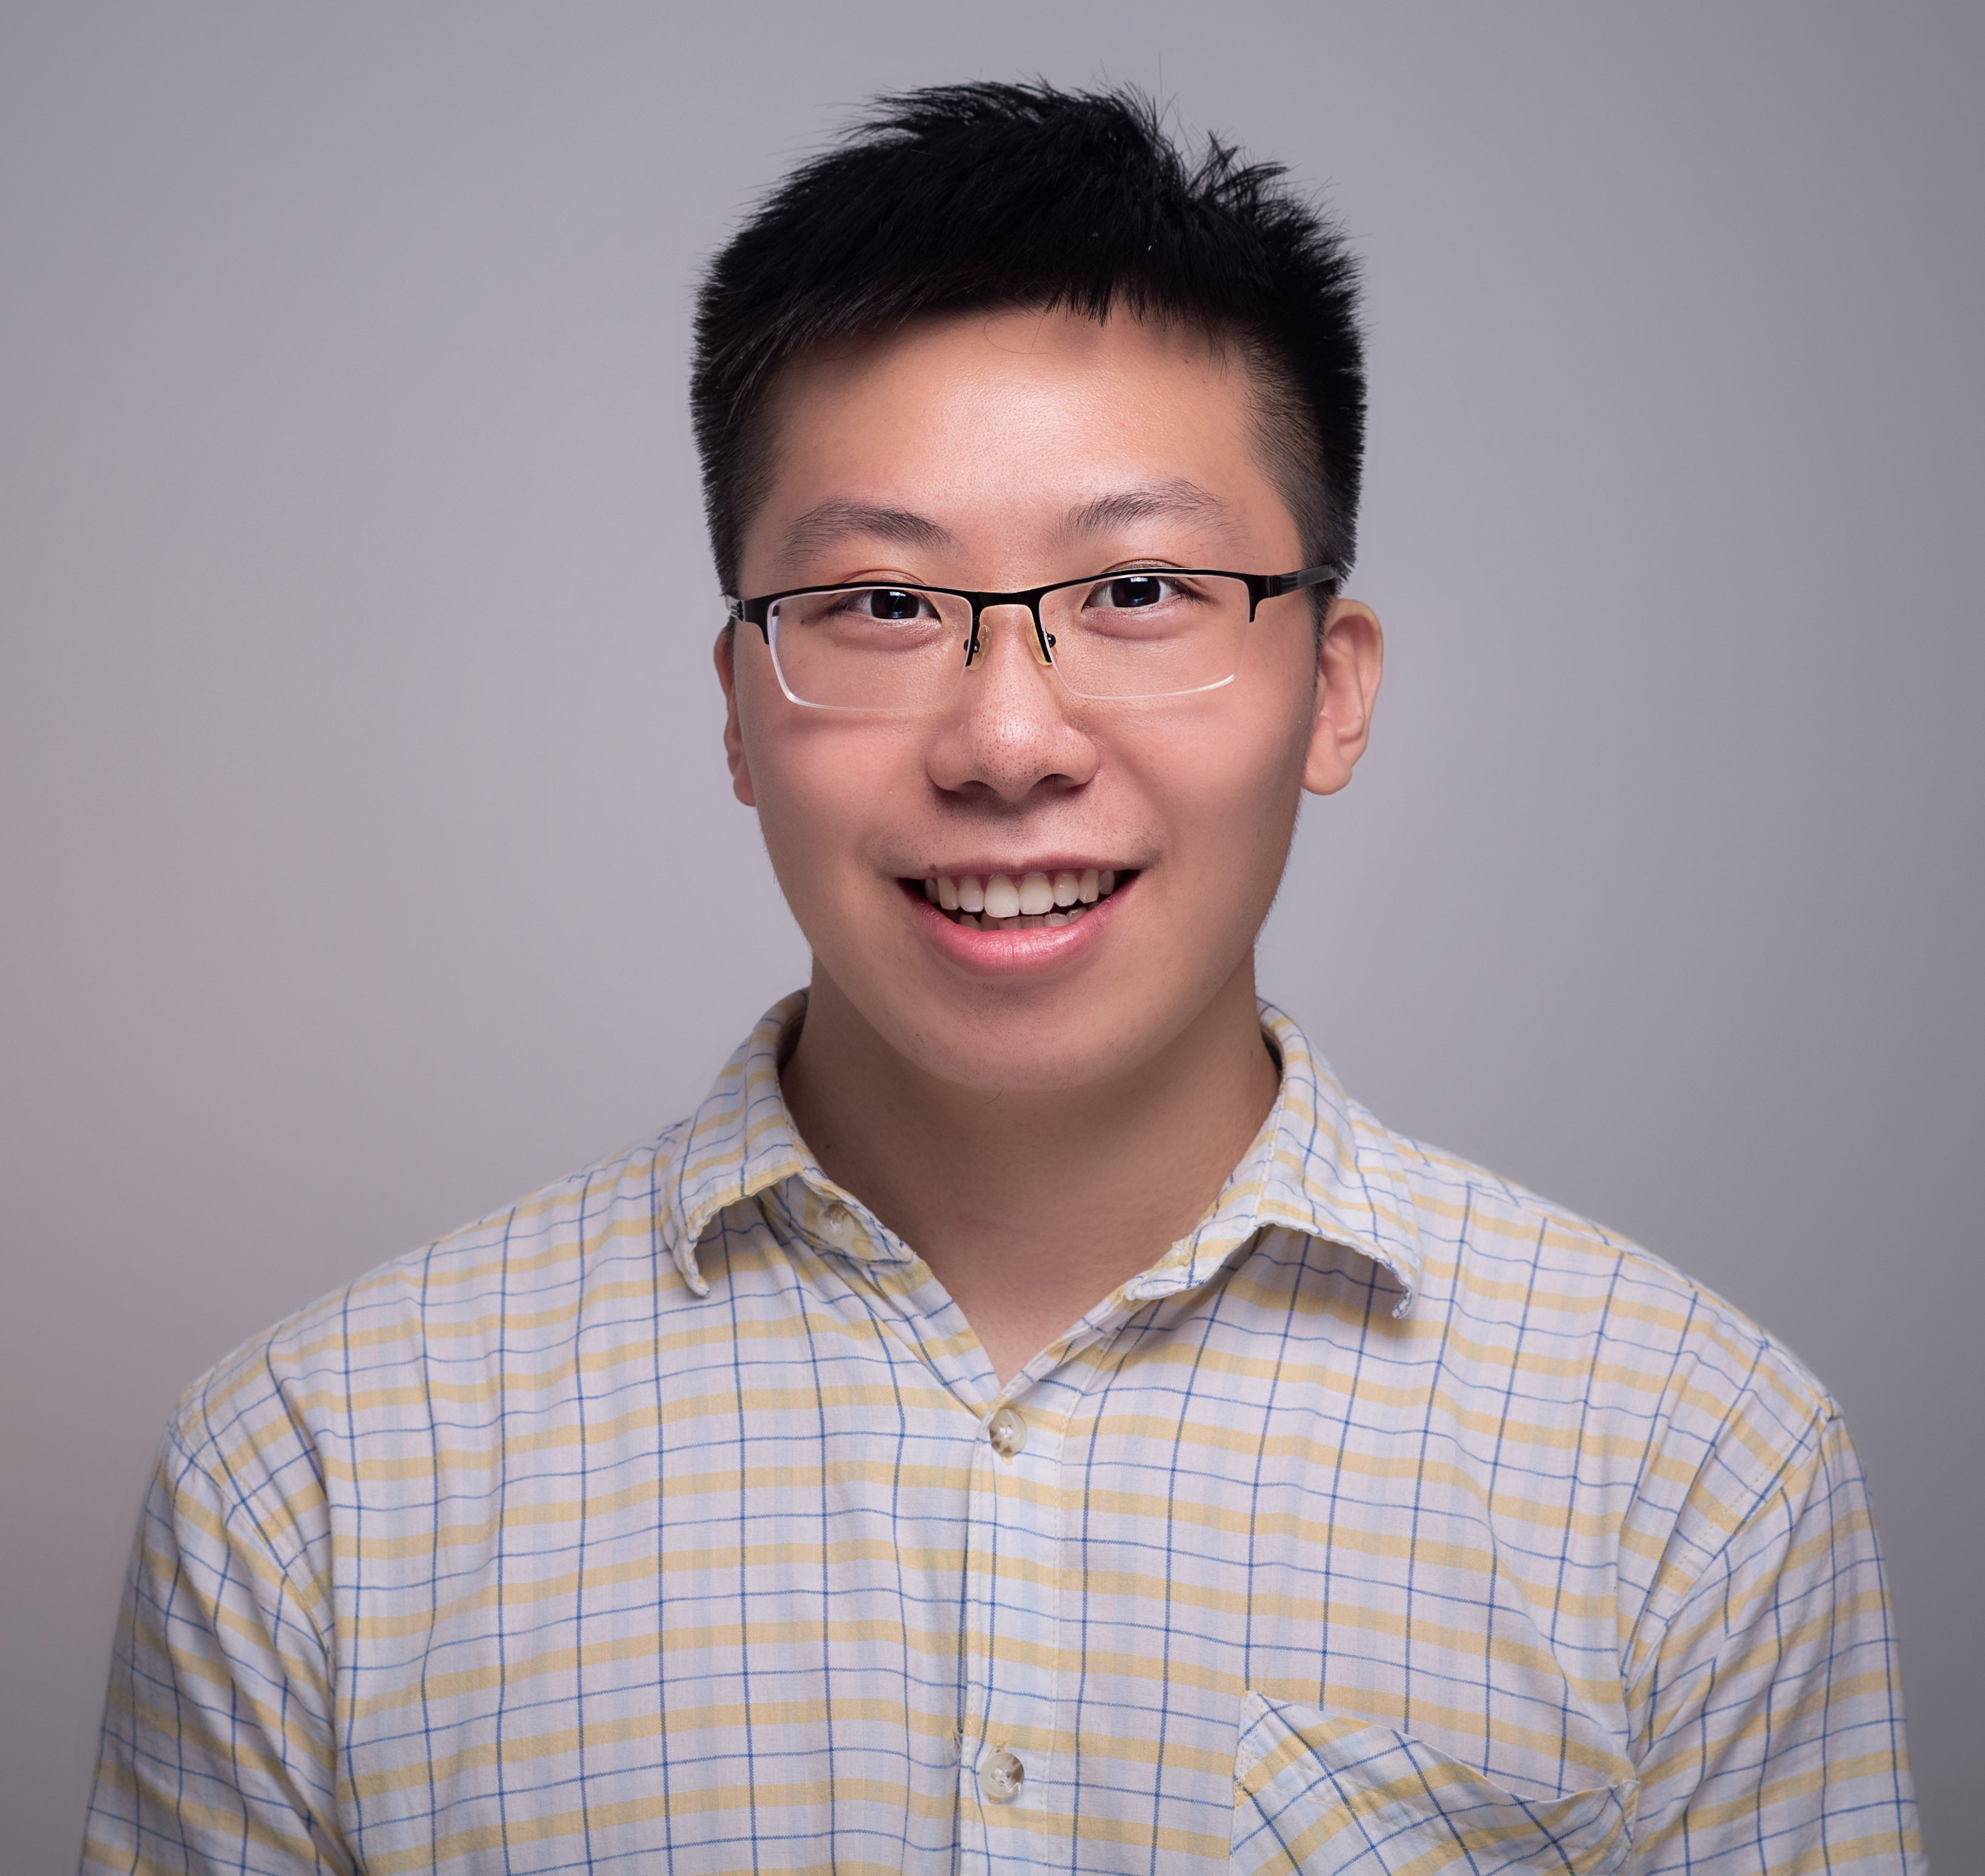
\includegraphics[width=1\textwidth]{cgb.jpg}
	\end{flushright}
\end{minipage}
\begin{minipage}[t]{0.07\textwidth}
\end{minipage}

%--------------
% Education
%--------------

\section{Education}

\datedsubsection{\textbf{Huazhong University of Science and Technology},\textbf{Computer Science and Technology},\textit{M.S. Candidate}}{Sep 2019 -- Sep 2025}
First-Class Academic Scholarship, Outstanding Communist Youth League Member

\datedsubsection{\textbf{Lanzhou University},\textbf{Computer Science and Technology},\textit{B.S.}}{Sep 2015 -- Jun 2019}
Ranked 2/69 (top 3\%), \textbf{National Scholarship}, Outstanding Graduate of Lanzhou University

%--------------
% Competitions & Awards
%--------------

\section{Competitions \& Awards}
\begin{itemize}[parsep=0.2ex]
  \item \textbf{ACM-ICPC Regional Silver Medal} (2018 Asia Regional Jiaozuo Silver, 2018 Asia Regional Qingdao Silver)
  \item \textbf{Higher Education Press Mathematical Modeling Competition, Undergraduate National Second Prize}
  % \item NOIP National First Prize (Guangdong Province Rank 7)
\end{itemize}

%--------------
% Internship Experience
%--------------


\section{Internship Experience}
% increase linespacing [parsep=0.5ex]
\ifboolexpr{test {\ifnumequal{\JobIndex}{0}} or test {\ifnumequal{\JobIndex}{1}} or test {\ifnumequal{\JobIndex}{2}} or test {\ifnumequal{\JobIndex}{3}} or test {\ifnumequal{\JobIndex}{4}} or test {\ifnumequal{\JobIndex}{5}} or test {\ifnumequal{\JobIndex}{6}} or test {\ifnumequal{\JobIndex}{7}} or test {\ifnumequal{\JobIndex}{8}}}{
	\datedsubsection{\textbf{UDrive Innovation \quad Intelligent Cockpit R\&D \quad C++ \quad Shenzhen}}{Aug 2025 -- Present}
}

\ifboolexpr{test {\ifnumequal{\JobIndex}{9}}}{
	\datedsubsection{\textbf{UDrive Innovation \quad Intelligent Cockpit R\&D \quad C++ \quad Shenzhen}}{Aug 2025 -- Oct 2025}
}

\begin{itemize}
	\item \textbf{Source Code Analysis}: Conducted in-depth studies of the occupant monitoring system (OMS) and driver monitoring system (DMS), focusing on facial and torso detection, facial image registration, and recognition algorithms.
	\item \textbf{Driver Hand Occupancy Detection Module}:
	\begin{itemize}
		\item \textbf{Problem Context}: In autonomous driving scenarios, drivers may struggle to quickly take over when both hands stay off the steering wheel for extended periods. The system must continuously detect hand occupancy status and plan safe takeover strategies. This project, developed jointly with an OEM, aimed to deliver a functional initial release.
		
		\item \textbf{Deep Learning Training, Inference, and Optimization}: Studied the full pipeline of lightweight hand and object detection models, from training to inference. Designed unit and integration tests, uncovering and fixing three technical defects.
		
		\item \textbf{Module Integration and System Design}: Integrated the hand occupancy module into OMS, completing pre- and post-processing for object detection. Redesigned the NMSMerger module and related data structures for hand and object detection to satisfy new scenario requirements.
	\end{itemize}
	\item \textbf{Automated Facial Registration/Recognition Testing}: Built automation scripts to batch process hundreds of video samples for facial registration and recognition, capturing failure cases for both registration and recognition.
\end{itemize}

\ifboolexpr{test {\ifnumequal{\JobIndex}{0}} or test {\ifnumequal{\JobIndex}{1}} or test {\ifnumequal{\JobIndex}{2}} or test {\ifnumequal{\JobIndex}{3}} or test {\ifnumequal{\JobIndex}{4}} or test {\ifnumequal{\JobIndex}{5}} or test {\ifnumequal{\JobIndex}{6}} or test {\ifnumequal{\JobIndex}{7}} or test {\ifnumequal{\JobIndex}{8}} or test  {\ifnumequal{\JobIndex}{9}}}{
	\datedsubsection{\textbf{Samsung China \quad Android SystemUI Development \quad Java, Kotlin \quad Guangzhou}}{Jun 2025 -- Jul 2025}
	\begin{itemize}
		\item \textbf{SystemUI Source Code Study}: Analyzed Android System UI source code with a focus on internal implementation of core components (Tiles, etc.).
		
		\item \textbf{Network Speed Indicator Design}: Investigated cross-version porting (Android 15 to 16) of the network speed indicator, covering dependencies on network state, toggle status, and screen on/off conditions, and produced UML sequence diagrams.
	\end{itemize}
}


%--------------
% Project / Algorithm Experience
%--------------

\section{Algorithm Experience}

\datedsubsection{\href{https://github.com/congmingyige/3D-Reconstruction-and-Quantitative-Analysis-of-Cerebral-Vasculature-under-Complex-Imaging-Conditions}{\textbf{Swin Transformer for Cerebral Vascular Segmentation, Skeletonization, and Network Analysis}}}{Jan 2024 -- May 2025}
\begin{itemize}
\item \textbf{Background}: Cross-disciplinary collaboration on brain vasculature research. Tsinghua University (Academician Zhuo Zhuang) led physical experiments; Huazhong University of Science and Technology (Academician Qingming Luo) led imaging with ex-vivo advantages (complete, fine-grained, spatially locatable data). Responsible for full-brain 3D vascular segmentation, skeletonization, and graph analysis. The task demands large receptive fields to capture injury signatures and must mitigate vessel breaks and noise.

\item \textbf{Methods}: Evaluated 19 supervised and zero-shot methods; a Swin Transformer with multi-level feature fusion, self-attention, and sliding windows performed best. Adapted Patch Embedding/Merging, Window Partition/Attention from 2D to 3D, added SENet channel attention to improve completeness, stacked $5 \times 1 \times 1$ and $3 \times 3 \times 3$ convolutions to enhance z-axis and small-scale connectivity, and incorporated lightweight denoising plus checkerboard artifact suppression. Delivered full segmentation, skeletonization, and visualization for 15 healthy or injured datasets every 2–3 days, enabling hemodynamic simulations and pre-clinical studies.

\item \textbf{Tech Stack}: PyTorch, NumPy, SciPy, SimpleITK/nibabel/libtiff (medical imaging), NetworkX (skeletonization and graph analysis), DataParallel, TensorBoard. Training on four NVIDIA A100 80GB GPUs; inference across fifteen NVIDIA RTX 5000 32GB servers. Portions are open-sourced on GitHub.

\end{itemize}

%--------------
% Conditional sections
%--------------

\ifthenelse{\equal{\JobIndex}{1}}{
	\section{Game Client Tool Experience}
}

\ifthenelse{\equal{\JobIndex}{2}}{
	\section{Development Experience}
}

\ifthenelse{\equal{\JobIndex}{3}}{
	\section{Development Experience}
}

\ifthenelse{\equal{\JobIndex}{4}}{
	\section{Client Development Experience}
}

\ifthenelse{\equal{\JobIndex}{5}}{
	\section{Development Experience}
}


%\ifthenelse{\equal{\JobIndex}{6}}{
%	\section{Development Experience}
%}

\ifthenelse{\equal{\JobIndex}{7}}{
	\section{Development Experience}
}

\ifthenelse{\equal{\JobIndex}{9}}{
	\section{Development Experience}
}

\ifboolexpr{test {\ifnumequal{\JobIndex}{1}} or test {\ifnumequal{\JobIndex}{2}} or test {\ifnumequal{\JobIndex}{3}} or test {\ifnumequal{\JobIndex}{4}} or test {\ifnumequal{\JobIndex}{5}} or test {\ifnumequal{\JobIndex}{7}} or test  {\ifnumequal{\JobIndex}{9}}}{
%\ifthenelse{\equal{\JobIndex}{2}}{

\begin{itemize}
	

\ifthenelse{\equal{\JobIndex}{1}}{
\item \textbf{Game Product Insights}:
	Deeply experienced titles such as \textit{Honkai: Star Rail}, \textit{Silksong}, and \textit{Mahjong Soul}, covering both free (story-driven) and paid (season pass, etc.) modes. Engage with gaming communities and peers to understand player sentiment and design philosophy, enabling analysis from both player and developer perspectives.
}

\ifboolexpr{test {\ifnumequal{\JobIndex}{1}} or test {\ifnumequal{\JobIndex}{2}} or test {\ifnumequal{\JobIndex}{3}} or test {\ifnumequal{\JobIndex}{4}} or test {\ifnumequal{\JobIndex}{5}} or test {\ifnumequal{\JobIndex}{7}} or test {\ifnumequal{\JobIndex}{9}}}{
\item \textbf{Mobile System Development}:
\begin{itemize}
	\item Studied Android System UI source with emphasis on porting the network speed indicator from Android 15 to 16, gaining architectural and state management knowledge.
	\item Extensive iOS ecosystem usage (iPhone, iPad, Mac, Watch, AirPods); researched iOS 16 features such as Liquid Glass and Snipaste (\href{https://github.com/congmingyige/Silksong-Sightseeing-Tour-Plugin}{\textbf{open-source}}).
	\item Accumulated hundreds of hours interacting with Apple Support to resolve issues and propose improvements, building deep insights into the iOS ecosystem.
\end{itemize}
}{}% end \ifboolexpr

\item \textbf{Engineering Tooling}:
\begin{itemize}
	\item Managed 14 workflows across 15 servers for deep learning projects via automation scripts, achieving efficient distributed scheduling and monitoring.
	\item Web literature translation (\href{https://github.com/congmingyige/translate-ignore-mathjax-available-for-google-translate}{\textbf{open-source}}): Built Power Automate + Tampermonkey scripts for bulk translation, including auto-scrolling, navigation, and math-aware translation bypass.
	\item GitHub Projects to PDF (\href{https://github.com/congmingyige/convert-multiply-html-files-to-pdf}{\textbf{open-source 1}} / \href{https://github.com/congmingyige/convert-multiply-markdown-files-to-pdf}{\textbf{open-source 2}}): Automated conversion of GitHub resources into PDFs, handling crawler limits, image loading, Markdown/HTML formatting, and auto-click flows.
	\item Resume LaTeX template (\href{https://github.com/congmingyige/Resume_LaTex}{\textbf{open-source}}): Dynamically optimizes margins and paragraph widths, supports multi-version resumes assembled via conditional logic, and auto-generates PDFs per target role.
\end{itemize}

\ifboolexpr{test {\ifnumequal{\JobIndex}{1}} or test {\ifnumequal{\JobIndex}{2}} or test {\ifnumequal{\JobIndex}{3}} or test {\ifnumequal{\JobIndex}{4}} or test {\ifnumequal{\JobIndex}{5}} or test {\ifnumequal{\JobIndex}{6}} or test {\ifnumequal{\JobIndex}{7}}  or test {\ifnumequal{\JobIndex}{9}}}{
\item \textbf{Full-Stack Development}:
\begin{itemize}
	\item Article reading web app with user interactions (\href{https://github.com/congmingyige/Article-reading-page-with-user-actions}{\textbf{open-source}}) (Front-end: Vue.js, HTML/CSS, JavaScript, HTTP; Back-end: Python, Django.db): CRUD for users/articles, reactions (like/favorite/comment), and author dashboards.
	\item Movie recommendation system (\href{https://github.com/congmingyige/Movie-Recommendation-System}{\textbf{open-source}}) (C, WinAPI for windowing, message handling, controls, drawing, file I/O): Rich GUI with scenario-based recommendations.
	\item Metro online ticketing system (\href{https://github.com/congmingyige/MTR-Online-Booking-System-with-Map}{\textbf{open-source}}) (Java, GUI, Socket, Thread, MySQL, algorithms): Multi-layer maps, zooming, multiple interaction modes, custom distance calculations.
\end{itemize}
}{}% end \ifboolexpr

\ifboolexpr{test {\ifnumequal{\JobIndex}{4}} or test {\ifnumequal{\JobIndex}{2}} or test {\ifnumequal{\JobIndex}{3}} or test {\ifnumequal{\JobIndex}{5}} or test {\ifnumequal{\JobIndex}{7}}  or test {\ifnumequal{\JobIndex}{9}}}{
	\item \textbf{Tooling Expertise}:
	\begin{itemize}
		\item \textbf{Development \& Debugging}: Proficient with Git, CMake, gdb, perf, valgrind, etc.
		%\item \textbf{Productivity}: Experienced with Notion, Everything, Dropbox, etc.
		\item \textbf{Data Management}: Responsible for petabyte-scale lab cluster backups using HDDs, tapes, optical media, etc.
	\end{itemize}
}{}% end \ifboolexpr

\ifthenelse{\equal{\JobIndex}{8}}{
	\item \textbf{Algorithms + Assembly + Databases}:
	\begin{itemize}
		https://github.com/congmingyige/Algorithm_with_Database_Assembly_HammingCode
		
	\end{itemize}
}

\ifthenelse{\equal{\JobIndex}{1}}{
\item \textbf{Innovation Practice \& Product Thinking}:
\begin{itemize}
	\item \textbf{High-Quality Tool Advocacy}: Frequent email discussions with Notion and Microsoft To Do teams on usage, bug reports, and feature proposals. Promote exceptional tools and contribute to ecosystem improvements.
	
	\item \textbf{Silksong Sightseeing Plugin Concept (\href{https://github.com/congmingyige/Silksong-Sightseeing-Tour-Plugin}{\textbf{open-source}})}:
		\begin{itemize}
			\item \textbf{Aesthetic Analysis \& Pain Points}: Highlights include birds bursting into flight as the protagonist passes and the exhilarating acceleration across open vistas. Pain points: RT acceleration halts near ledges/water exits, and high difficulty deters players seeking exploration only.
			
			\item \textbf{Technical Design}: Planned UI and controls (sliders for speed, directional/boost inputs). Explored three approaches for moving from A to B: Unity engine background manipulation, video frame control, and game mods/hooks.
			
			\item \textbf{Implementation Details}: For the mod-based approach, combined invincibility, infinite resources, double jump, one-hit kill, and character swap mods. Designed short- and long-distance auto-travel plus branch-aware path planning. Leveraged invincibility to reduce dev difficulty, speed mods to cut wait times, and auto return-to-start to minimize user input.
		\end{itemize}
	
	\item \textbf{Reconfigurable Mahjong Tile Accessories}:
	\begin{itemize}
		\item Used magnetic attraction between adjacent tiles for flexible yet firm compositions (e.g., East-South-West-North, dragon tiles, red fives, custom patterns like AA2333 or date/weather motifs) with removable stickers.
		
		\item Evaluated external/internal magnets and 3D shells; chose ultra-thin external magnets for aesthetics after weighing cost, time, and complexity.
		
		\item Performed load and geometry analysis to determine ideal lanyard lengths, selected premium cords/hooks, and applied odorless, colorless adhesive for daily usability.
	\end{itemize}
\end{itemize}
}

\end{itemize}% Close itemize opened near line 315
}{}% End \ifboolexpr

\ifboolexpr{test {\ifnumequal{\JobIndex}{2}} or test {\ifnumequal{\JobIndex}{3}} or test {\ifnumequal{\JobIndex}{6}} or test {\ifnumequal{\JobIndex}{10}}}{
	\section{Graph Theory (Routing) Experience}
	\begin{itemize}
		\item \textbf{Algorithms Mastered/Familiar}: 
		\begin{itemize}
			\item Fundamentals: DFS/BFS, Dijkstra, Bellman-Ford, SPFA, Kruskal, Prim, Topological Sort, Tarjan, Max-Flow, Hamiltonian Graphs, A*
			\item Related Algorithms: LCA, heavy-light decomposition, tree decomposition, tree diameter, segment trees, bitmask DP, dynamic programming, meet-in-the-middle
			\item Advanced: TSP, VRP, reinforcement learning, approximation algorithms
		\end{itemize}
		\item \textbf{Blogging}: Authored 500+ posts covering graph algorithms and research work.
		\item \textbf{Problem Setting} (\href{https://github.com/congmingyige/ACM-ICPC_Create_Algorithm_Problems_by_XiaoC}{\textbf{open-source}}): Created and verified DFS/BFS/multi-source BFS/Dijkstra/Hamiltonian graph/flow problems.
		\item \textbf{Applications}: Designed a mobile robot trash bin with dual rollers for waste collection.
	\end{itemize}
}{}% End \ifboolexpr

% {
% \ifthenelse{\equal{\JobIndex}{9}}{
	% 	\section{About Yajiang}
	% }
% 
% 	\begin{itemize}
	% 	\item 123
% \end{itemize}
% }

\ifthenelse{\equal{\JobIndex}{9}}{
	\section{Group Activities}
	\begin{itemize}
	\item Served as badminton coordinator in the grad lab for two years, booking courts weekly and organizing annual events.
	\item Organized and participated in the Lanzhou University programming contest three times, covering problem setting, validation, and logistics.
	\end{itemize}
}

\end{document}
